

\section{Caratteristiche della Simulazione}\label{Parte B}
Prima di studiare le caratteristiche del sistema fisico in esame è necessario analizzare le proprietà degli algoritmi che intendono simularlo.
Per prima cosa si può cominciare con un'analisi di tipo qualitativo del comportamento del sistema, limitandosi ad osservare immagini delle configurazioni di un reticolo finito di spin nella sua evoluzione termica caotica.
   \begin {figure}[h!]
      \begin{center}
      	\caption[1) Preliminari\_Snap\_Metro.cpp $\quad / \quad$2) Preliminari\_Snap\_Cluster.cpp ]{Raffreddamento a $\beta = 1,2 $ con algoritmo di Metropolis(sopra) e MultiCluster (sotto).}\label{fig:3}
        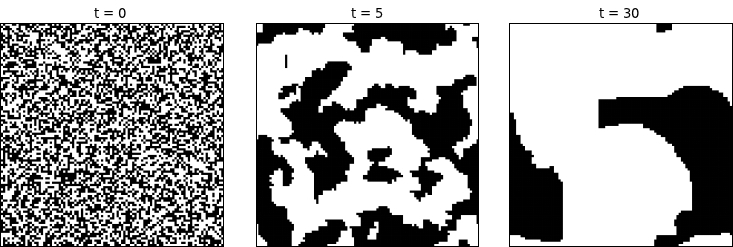
\includegraphics[scale=0.5]{Immagini/Metro_raffreddamento.jpg}
        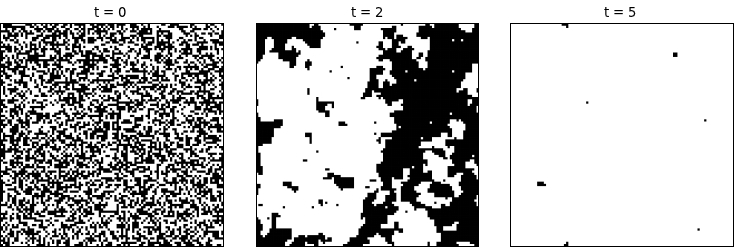
\includegraphics[scale=0.5]{Immagini/Cluster_raffreddamento.jpg}
      \end{center}
    \end {figure}     
\bigskip \newline   
Nella figura (\ref{fig:3}) è possibile osservare tre istantanee del raffreddamento (termalizzazione a $\beta>1$ di una configurazione disordinata) del sistema con $L=100$ a partire da una configurazione casuale( $t$ rappresenta il numero di step dell'algoritmo effettuato, i quadratini bianchi rappresentano spin con orientazione $+1$ e i neri $-1$) realizzato prima con l'algoritmo di Metropolis e poi con l'algoritmo a MultiCluster. \newline
E' evidente come l'algoritmo di Swenden-Wang porti ad una configurazione ordinata molto più rapidamente dell'algoritmo di Metropolis che invece presenta delle grandi isole di spin opposto anche dopo molti passi.
\begin{figure}[htbp]
     \begin{minipage}{0.8\textwidth}
Il fenomeno è dovuto alla definizione dell'algoritmo. Per temperature molto basse le fluttuazioni termiche sono quasi totalmente smorzate per cui la probabilità di essere invertito per uno spin situato lungo il bordo di una grande isola sono praticamente nulle. 
Gli spin sul bordo dell'isola , infatti, sono adiacenti a 3 spin paralleli che a loro volta hanno come primi vicini altri 3 o più spin della medesima orientazione, pertanto il flip di uno qualsiasi di essi porterà ad una configurazione ad energia maggiore( da scartare) e la "barriera" resterà immutata (vedere figura ~\ref{fig:bariera spin}).
     \end{minipage}\hfill
     \begin{minipage}{0.2\textwidth}
      \centering
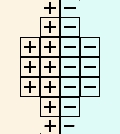
\includegraphics[width=0.58\textwidth]{Immagini/bariera.jpg}
       \caption[Bariera di Spin.]{}\label{fig:bariera spin}
     \end{minipage}
   \end{figure}
\bigskip
     \begin {figure}[h!]
      \begin{center}
		\caption{Riscaldamento a $\beta = 0,008 $ }\label{fig:riscaldamento}
        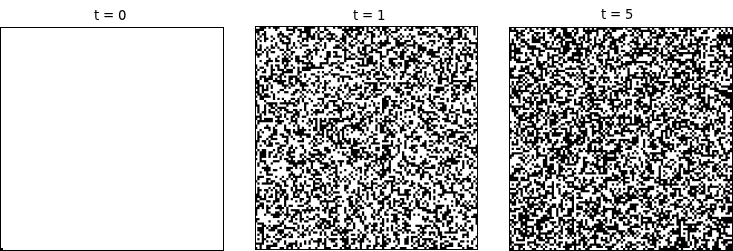
\includegraphics[scale=0.5]{Immagini/Metro_riscaldamento.jpg}
      \end{center}
\end {figure}
\newline Per quanto riguarda il riscaldamento del sistema (termalizzazione a $\beta\ll1$ di una configurazione molto ordinata) non si nota nessuna sostanziale differenza tra il comportamento dei due algoritmi come si può osservare dalla figura (\ref{fig:riscaldamento}).
\bigskip \newline 
La "dinamica" determinata da i due algoritmi si differenzia fortemente alle basse temperature. 
L'algoritmo a Multi-Cluster, con la sua probabilità $1:2$ di inversione dei cluster, fa si che uno stato ordinato oscilli continuamente tra configurazioni con spin totale opposto (per questo sarà necessario definire osservabili \emph{improved}), questo non deve soprendere perchè si tratta di configurazioni con la stessa energia e quindi equiprobabili.
L'algoritmo di Metropolis discrive invece una dinamica più "naturale", il sistema ferromagnetico tende a sviluppare un'orientazione magnetica specifica man mano che viene raffreddato.


\subsection{Tempo di Esecuzione}
L'algoritmo di Swenden-Wang non presenta il problema della formazione di barriere ma la maggiore complessità del codice necessario per implementarlo comporta una maggiore lentezza di esecuzione.
     \begin {figure}[h!]
      \begin{center}
		\caption[Preliminari$\_$TempoEsecuzione.cpp]{Tempo di esecuzione di un passo evolutivo in funzione della taglia del reticolo.}\label{fig:t_esec}
        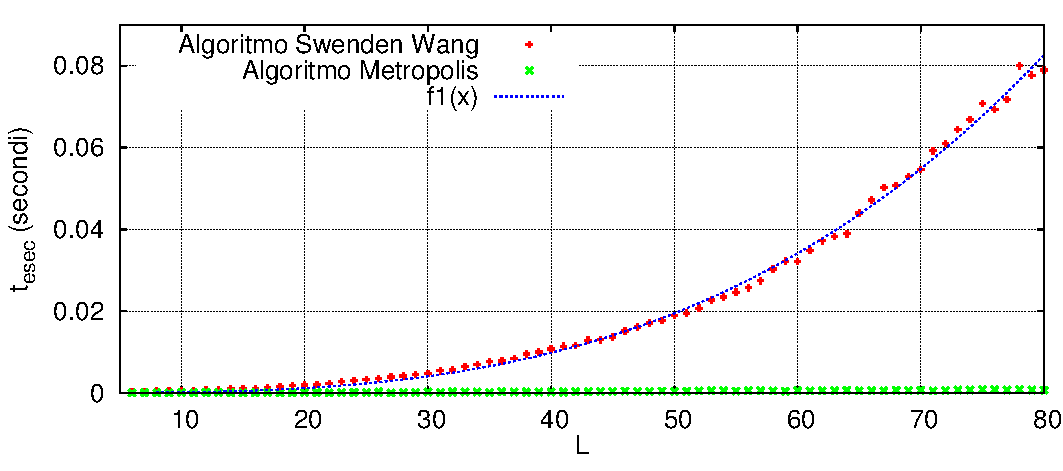
\includegraphics[scale=0.65,]{Immagini/ParteB/TempoEsecuzione}
		\newline \footnotesize  $L = 80\quad T=T_{crit}$
      \end{center}
    \end {figure} 
Nella figura (\ref{fig:t_esec}) è messo a confronto il tempo medio di esecuzione di un singolo step per i due algoritmi al variare del valore della taglia del reticolo $L$ (numero di spin su una riga)\footnote{Codice sorgente : \emph{"Preliminari\_TempoEsecuzione.cpp"}}.
E' evidente come l'algoritmo a Multi-Cluster sia molto più lento e il tempo di esecuzione cresca molto più rapidamente al variare di $L$ (nel grafico è presente un fit con una funzione $\propto L^3$)\footnote{Siccome l'algoritmo di metropolis prevede un test per ogni nodo ci si aspetta che il tempo di esecuzione cresca come $L^2$.}.


\subsection{Tempo di Termalizzazione}
Con \emph{Tempo di Termalizzazione} si intende il numero di passi dopo di cui la distribuzione di probabilità degli elementi della catena di Markov può essere considerata equivalente alla distribuzione limite.
\newline
Questo tempo si può stimare in modo qualitativo osservando i grafici che danno il valore degli osservabile microscopici (definiti sulla singola configurazione) come ad esempio lo spin totale per numero di nodi($M$) e la densità di energia($H$), nell'evoluzione della configurazione lungo la catena di Markov. \newline
Nei grafici viene posto in ordinata il valore istantaneo dell'osservabile $O(\phi_k)$ e in ascissa il numero di passi dell'algoritmo applicati ad un generico stato iniziale (quindi $k$). 
Il "tempo" in cui i grafici relativi ad una stessa $\beta$ di termalizzazione, ma con diversa configurazione iniziale, convergono e cominciano ad oscillare attorno ad uno stesso valore (che presumibilmente sarà il valore d'aspettazione $\langle O \rangle$) è una buona stima operativa del tempo di termalizzazione.
Dalle figure si può determinare una stima approsimativa per i tempi termalizzazione ($\tau_{eq}$) minimi consigliati:
\begin{center}
\begin{tabular}{|l|c|}
  \hline
  $\tau_{eq}$ Metropolis & $\sim 150$ step per sito \\
  $\tau_{eq}$ Multi Cluster & $\sim 30$ step\\ 
  \hline
\end{tabular}
\end{center}

\clearpage

\begin{figure}[!h]
\centering
\caption[ParteB$\_$Termal$\_$Metro.cpp ]{\footnotesize Termalizzazione Metropolis ( $L=100$)}\label{fig: termo_metro}
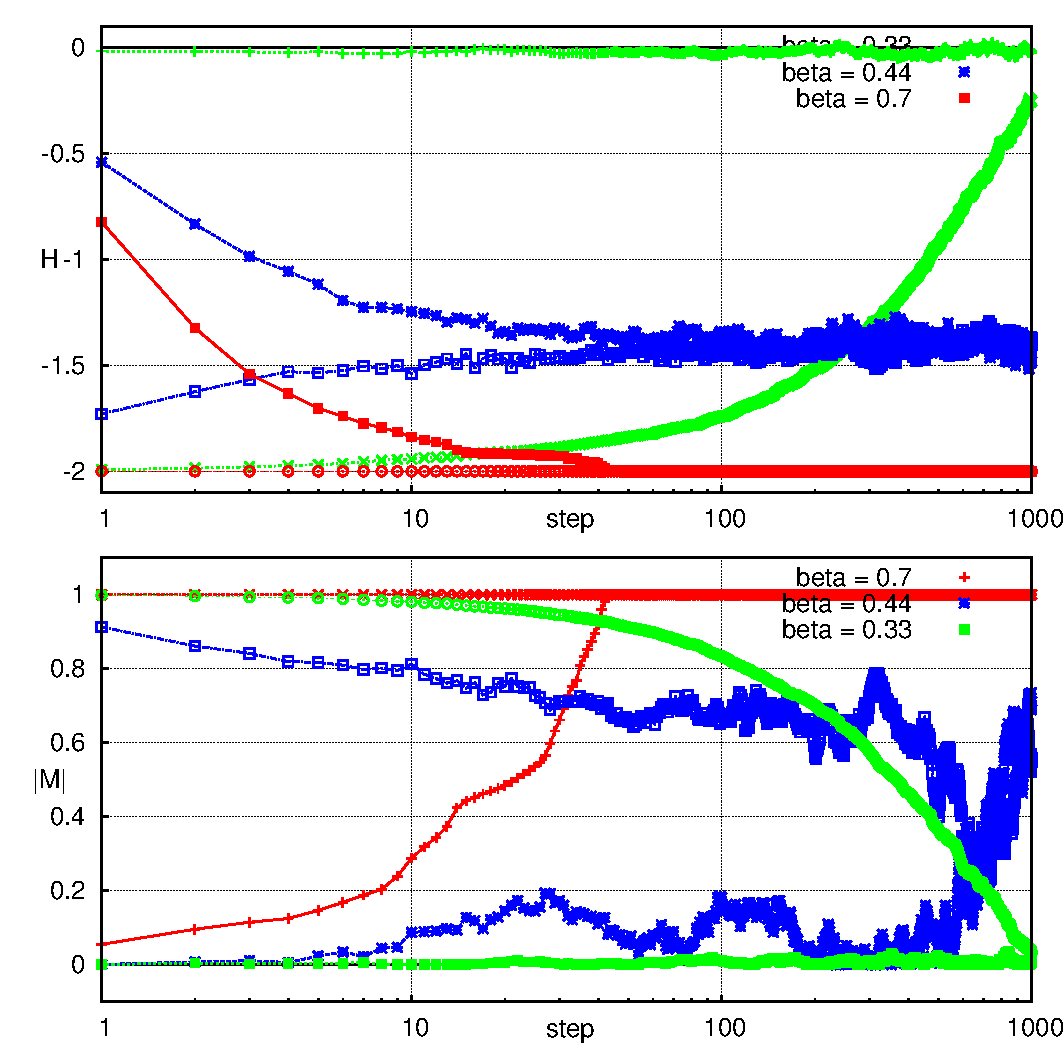
\includegraphics[scale=0.65]{Immagini/ParteB/Metro_Termal}
\caption[ParteB$\_$Termal$\_$Cluster.cpp ]{\footnotesize Termalizzazione Multi-Cluster ( $L=100$)}\label{fig: termo_cluster}
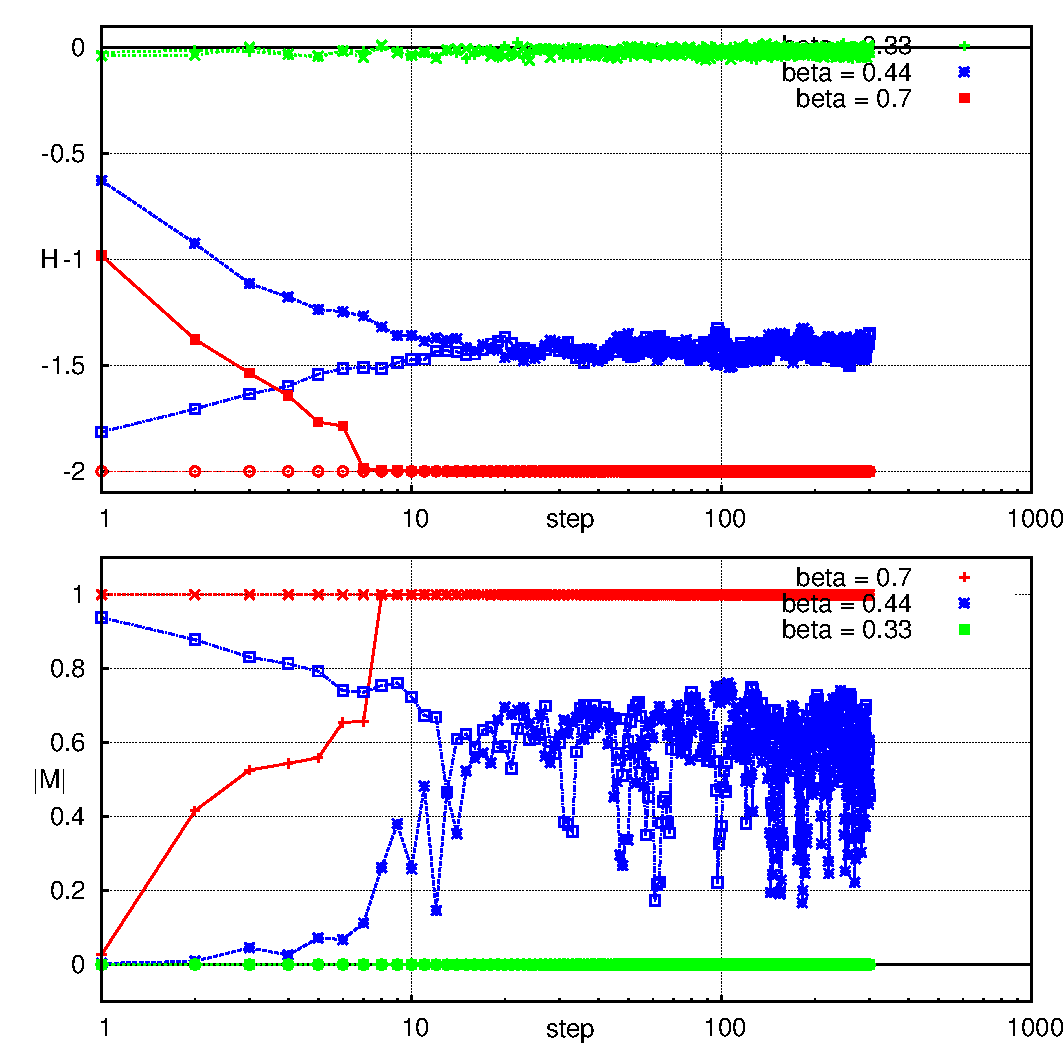
\includegraphics[scale=0.65]{Immagini/ParteB/Cluster_Termal}
\end{figure}


I grafici analizzati sono la figura (\ref{fig: termo_metro}) relativamente alla termalizzazione degli osservabili $H$ e $M$ tramite algoritmo di Metropolosi e la figura (\ref{fig: termo_cluster}) per l'algoritmo di SwendenWang.\newline
Si osserva che:
\begin{itemize}
\item Il numero di step necessari alla termalizzazione dipende fortamente dalla temperatura finale. Intorno a $\beta \simeq 0.44$ (temperatura critica) la termalizzazione diventa sensibilmente più lunga, l'effetto è molto più evidente per l'algoritmo di Metropolis in quanto soffre di una rapida divergenza del \emph{Tempo di Autocorrelazione}.
\item Il tempo di termalizzazione per il raffreddamento con l'algoritmo di Metropolis soffre il fenomeno della barriera di spin.
\end{itemize}

\subsection{Tempo di Autocorrelazione}
Il \emph{tempo di correlazione} è una misura del "tempo" (numero di passi di evoluzione) necessario a portare una configurazione del sistema in un'altra configurazione significativamente differente dalla prima.
Per misurarlo è necessario studiare l'andamento della funzione di autocorrelazione del sistema $CA(t)$ relativa ad un generico osservabile $O$.\newline
Per un sistema di Ising discreto, $\textrm{CA}(t)$ viene definita su una catena di Markov $(\phi_0, \ldots, \phi_{K} )$ come segue:
\begin{equation}
\begin{split}
\textrm{CA}(t) =& \dfrac{1}{K-t} \sum_{t'=0}^{K-t}O(t')O(t+t') - 
	  \biggr(\dfrac{1}{K-t}\sum_{t'=0}^{K-t}O(t')\biggr)
	  \biggr( \dfrac{1}{K - t}\sum_{t'=0}^{K-t}O(t'+t) \biggr) \\
	  =& \langle O(t_0)O(t)\rangle - \langle O(t_0) \rangle \langle O(t) \rangle
\end{split}
\end{equation}
(perchè il valore sia statisticamente significativo il massimo valore di $t$ su cui si valuta l'autocorrelazione dovrà essere molto minore del numero di configurazioni campionate $K$).\newline
L'andamento atteso della funzione di autocorrelazione è a decadimento esponenziale:
\begin{equation}
	\textrm{CA}(t) \propto e^{-t/\tau}
\end{equation}
la scala caratteristica $\tau$ del decadimento è ciò che formalmente si definisce \emph{tempo di autocorrelazione}.

Per come è definito $\tau$ corrisponde al valore di $t$ per cui $\textrm{CA}(t)/\textrm{CA}(0) = e^{-1} \simeq 0.37$ quindi quando $t = 2\tau$ la funzione di correlazione assume un valore molto piccolo e la configurazione può essere considerata scorrelata nel senso intuitivo di "dissimile".
\begin{figure}[!h]
\centering
\caption[ParteB$\_$Autocorrelazione$\_$CAvst$\_$Cluster.cpp ]{Autocorrelazione di $H$ - Algoritmo Swenden-Wang }\label{fig: Cluster_CAvst}
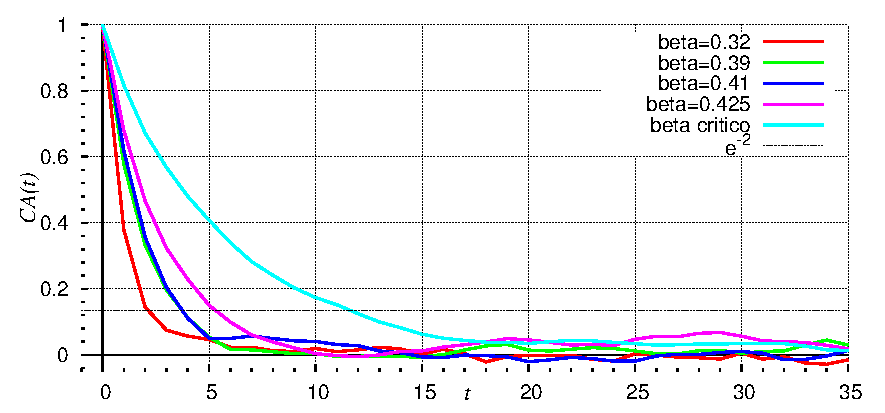
\includegraphics[scale=0.75]{Immagini/ParteB/Cluster_CAvst}
\newline \footnotesize L=100, $K = 8000$
\end{figure}
\begin{figure}[!h]
\centering
\caption[ParteB$\_$Autocorrelazione$\_$CAvst$\_$Metro.cpp ]{Autocorrelazione di $H$ - Algoritmo Metropolis }\label{fig: Metro_CAvst}
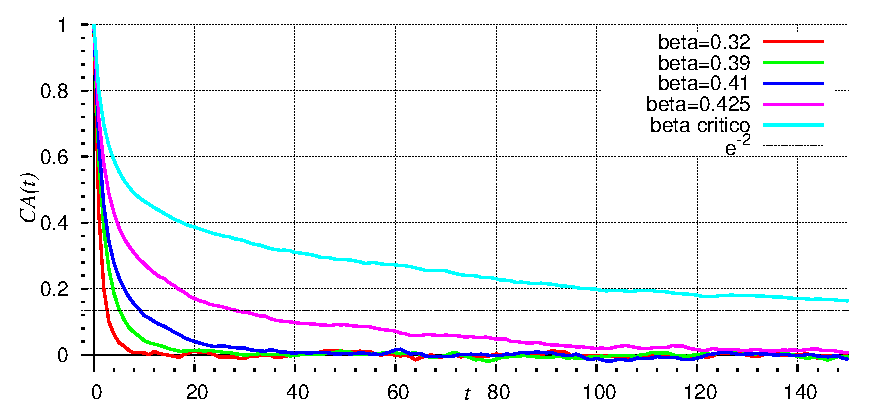
\includegraphics[scale=0.75]{Immagini/ParteB/Metro_CAvst}
\newline \footnotesize L=100, $K = 100000$
\end{figure}
\newline
Nei grafici (\ref{fig: Metro_CAvst}) e (\ref{fig: Cluster_CAvst}) è rappresentato l'andamento della funzione di correlazione normalizzata( $\textrm{CA}(t)/\textrm{CA}(0)$) relativa all'osservabile $H$ al variare del numero di step evolutivi $t$, calcolata per i due algoritmi.\newline
Si osserva che:
\begin{itemize}
\item Il valore di autocorrelazione decade molto rapidamente ma altrettanto rapidamente l'andamento diventa molto rumoroso, rendendo un ipotetico fit esponenziale poco significativo per la stima del tempo di autocorrelazione.
Osservando i grafici è possibile dare "ad occhio" una stima rozza di $2\tau$ come punto in cui la correlazione è quasi 0 ( quando $t=2\tau$ si ha  $\textrm{CA}(t)/\textrm{CA}(0)= e^{-2} \simeq 0.1$).

\item Dalla definizione segue che il valore del tempo di correlazione regola la convessità della curva, al crescere di $\tau$ l'andamento della funzione di autocorrelazione tendera ad appiattirsi sempre di più verso una retta.
Detto questo è evidente la dipendenza di $\tau$ dalla temperatura: il tempo di correlazione cresce all'aumentare di $\beta$, ha un picco alla temperatura critica e dopo tende di nuovo a diminuire.

\item Per lo stesso criterio di prima si può affermare che il tempo di autocorrelazione è molto minore per l'algoritmo di Swenden-Wang rispetto all'algoritmo di Metropolis.
\end{itemize}

\subsubsection*{$\tau$ Integrale}$\\$
Un secondo criterio per calcolare il tempo di correlazione è il metodo integrale basato sulla semplice osservazione che:
\begin{displaymath}
\dfrac{\textrm{CA}(t)}{\textrm{CA}(0)}\simeq e^{-t / \tau} \quad \Longrightarrow \quad \int_{0}^{\infty}\dfrac{\textrm{CA}(t)}{\textrm{CA}(0)} \simeq \int_{0}^{\infty} e^{-t / \tau} = \tau
\end{displaymath}
Per la simulazione computazionale il tempo è discretizzato in passi e l'integrale di prima dovrà essere calcolato come una somma, ovvero:
\begin{equation}
	\sum_{t=0}^{\infty}\dfrac{\textrm{CA}(t)}{\textrm{CA}(0)} \simeq \tau
\end{equation}	
che non è altro che il calcolo dell'integrale delle funzioni di correlazione mostrate prima calcolato con il metodo dei rettangoli. Per via dei limiti computazionali la sommatoria dovrà essere troncata ad un valore $t_{max}$, scelto sufficientemente grande da permettere di trascurare i contributi a tempo successivi senza determinare un eccessivo errore.
\begin{figure}[!h]
\centering
\caption[ParteB$\_$TauvsX$\_$Metro.cpp $\quad$e$\quad$ ParteB$\_$TauvsX$\_$Cluster.cpp]{Andamento $\footnotesize \tau_{int}$ vs $X= \dfrac{\beta-\beta_c}{\beta_c}$}\label{fig: TauHvsX}
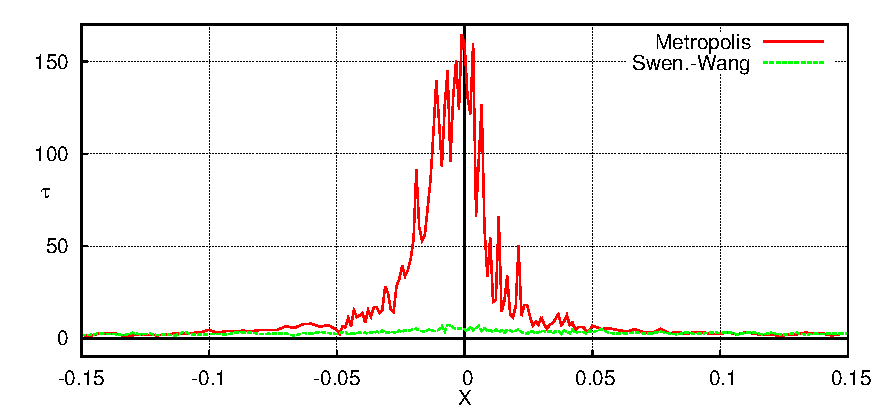
\includegraphics[scale=0.75]{Immagini/ParteB/TauHvsX}
\newline \footnotesize $L=100\, , \quad K_{metro} = 51000\, , \quad (t_{max})_{metro} = 1000\, , \quad K_{cluster} = 5100\, , \quad (t_{max})_{cluster} = 100 $
\end{figure}
\newline Stampando i valori di $\tau_{int}$ al variare di $X=(\beta-\beta_c)/\beta_c$ (vedere figura ~\ref{fig: TauHvsX}) si ha una conferma immediata  della divergenza del tempo di autocorelazione in prossimità della temperatura critica ( X = 0).
Dal grafico è inoltre evidente la forte dipendenza del valore del tempo di correlazione dall'algoritmo di simulazione usato.
\medskip
In conclusione, dalle simulazioni effettuate per generare i grafici (\ref{fig: Cluster_CAvst}) e (\ref{fig: Metro_CAvst}) risultano le seguenti stime per i valori del tempo di autocorrelazione:
\begin{center}
\begin{tabular}{ | c| c c| c c|} 
\hline
$\beta$		& \multicolumn{2}{|c|}{$2\tau$ "ad occhio" } & \multicolumn{2}{|c|}{$\tau$" integrale" } \\
\hline 
	  & metropolis & multicluster & metropolis & multicluster \\
 0,32 & $\sim$3    & $\sim$2,18   & $\sim$1,95 & $\sim$1.96   \\
 0,39 & $\sim$5,5    & $\sim$3,8   & $\sim$4 & $\sim$2.8   \\
 0,41 & $\sim$9.2    & $\sim$3,8   & $\sim$5,4 & $\sim$2.06   \\
 0,425& $\sim$28.5    & $\sim$5,3   & $\sim$15,6 & $\sim$4.16   \\
 $\beta_c$ & $\sim$223    & $\sim$11,5   & $\sim$112,2 & $\sim$7.5   \\
 \hline 
\end{tabular}
\end{center}



\subsubsection*{Dipendenza di $\tau$ da L}
Resta da stabilire quanto il valore del tempo di autocorrelazione dipenda dalla dimensione $L$ del sistema simulato.
Si procede come prima, stampando l'andamento della funzione di correlazione normalizzata con temperatura fissata al valore critico ma a diversi valori della taglia del reticolo $L$.

\begin{figure}[!h]
\centering
\caption[ParteB$\_$Tc$\_$TauvsN$\_$Cluster.cpp]{Autocorrelazione di $H$ -\footnotesize  Algoritmo Swenden-Wang, vari $L$}\label{fig: Cluster_Tc_CAvst}
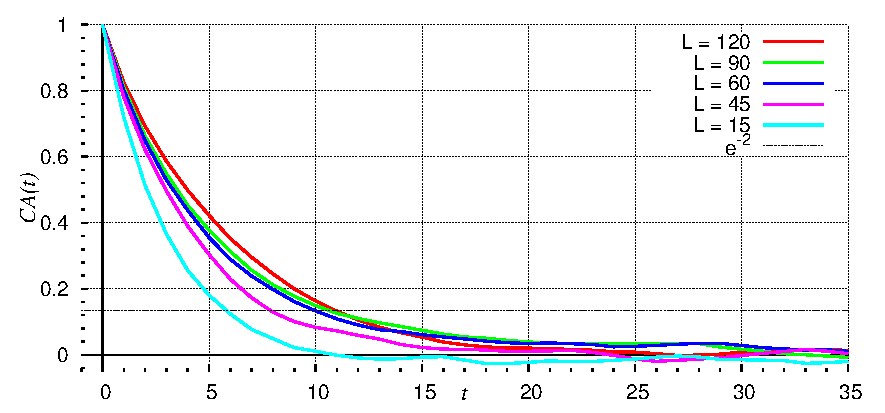
\includegraphics[scale=0.75]{Immagini/ParteB/Cluster_Tc_CAvst}
\newline \footnotesize $\beta = \beta_c$, $K = 10200$
\end{figure}

\begin{figure}[!h]
\centering
\caption[ParteB$\_$Tc$\_$TauvsN$\_$Metro.cpp]{Autocorrelazione di $H$ -\footnotesize  Algoritmo Metropolis, vari $L$}\label{fig: Metro_Tc_CAvst}
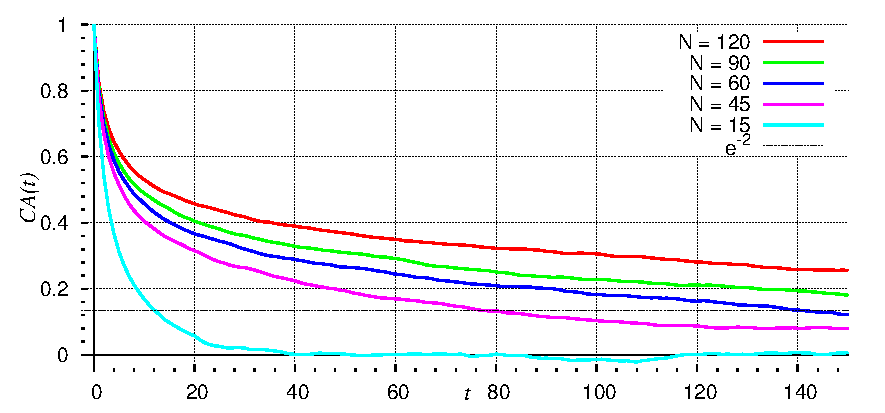
\includegraphics[scale=0.75]{Immagini/ParteB/Metro_Tc_CAvst}
\newline \footnotesize $\beta = \beta_c$, $K = 10200$
\end{figure}
Si evince dai grafici che per ogni reticolo il valore massimo del tempo di correlazione (valore in prossimatità della temperatura critica) dipende dalla taglia del sistema e aumenta con esso. 
Per studiare la divergenza del tempo di correlazione è possibile introdurre un esponente \emph{critico (dinamico)}\cite{Newman2001} $z$ che descive l'andamento del tempo di correlazione alla temperatura critica:
\begin{equation}
\tau \sim L^z
\end{equation}
Stampando $\tau_{int}$ (figura \ref{fig: Tau_Tc_L}) in funzione di $L$ a $\beta_c$ fissato ed eseguendo un fit lineare in scala logaritmica dei dati si può ottenera una stima di tali esponenti critici.

\begin{figure}[!h]
\centering
\caption[ParteB$\_$Tc$\_$TauvsN.cpp ]{Andamente del tempo di autocorrelazione integrale in funzione di $L$.}\label{fig: Tau_Tc_L}
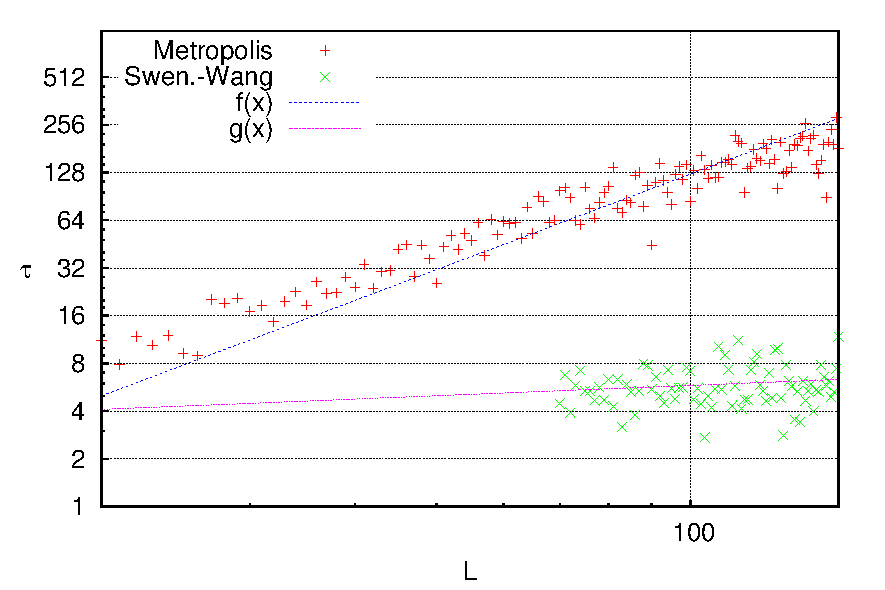
\includegraphics[scale=0.75]{Immagini/ParteB/TauHvsN}
\newline \footnotesize L=100, $K = 100000$
\end{figure}

La disposizione dei dati non è particolarmente ordinata ( era già visibile nelle figure ~\ref{fig: Cluster_CAvst} e ~\ref{fig: Metro_CAvst} l'andamento della funzione di correlazione diventa rapidamente molto rumoroso) ma è possibile dedurre dei valori approssimativi per l'esponente dinamico:
\begin{center}
\begin{tabular}{ | c | c |} 
\hline
$z_{metro}$ & $\sim$ 2 \\
\hline 
$z_{cluster}$ & $\sim$ 0.2 \\
\hline 
\end{tabular}
\end{center}

\subsection{Conclusioni}
Dalle analisi precedenti emergono le carateristiche fondamentali dei due algoritmi:
\begin{itemize}
\item \underline{Metropolis}: Soffre di una grande divergenza di $\tau_{eq}$ e del $\tau_{correlazione}$ in prossimità della $\beta$ critica. Questo comporta che per ottenere una statistica di configurazioni  significativa intorno a questa temperatura sia necessario evolvere il sistema un numero di volte molto maggiore di quanto siano i dati effettivamente ottenuti (oppure di campionare i dati dopo intervalli d'evoluzione più lunghi). 
In compenso un singolo passo dell'algoritmo richiede un tempo di esecuzione molto più basso rispetto all'algoritmo a multicluster, soprattutto per le taglie del reticolo grandi.
\item \underline{Swenden-Wang}: Il valore basso di $\tau_{correlazione}$ lo rende estremamente efficente per lo studio del sistema intorno alla temperatura critica. Anche il $\tau_{eq}$ si mantiene basso ad ogni temperatura, ciò lo rende l'algoritmo ideale per portare il sistema a termalizzazione prima di una misurazione. Il grande problema è il tempo di esecuzione e la sua forte dipendenza da $L$, infatti per simulare un sistema di taglia $L=100$ sono necessarie diverse ore. 
\end{itemize}
Per studiare i valori d'aspettazione degli osservabili macroscopici sul sistema sarà necessario sfruttare i vantaggi di entrambi gli algoritmi: l'algoritmo a multicluster verrà sfruttato per simulare la zona critica negli altri casi si farà uso dell'algoritmo di Metropolis.
\newline
Bisogna notare però che a temperature alte i due algoritmi danno valori diversi per l'osservabile di magnetizzazione assoluta( figura ~\ref{fig: Confronto_M_andamento} ).

\begin{figure}[htbp]
     \begin{minipage}{0.5\textwidth}
\centering
\caption[Preliminari$\_$Magnetizzazione.cpp ]{\footnotesize Osservabile di magnetizzazione}\label{fig: Confronto_M_andamento}
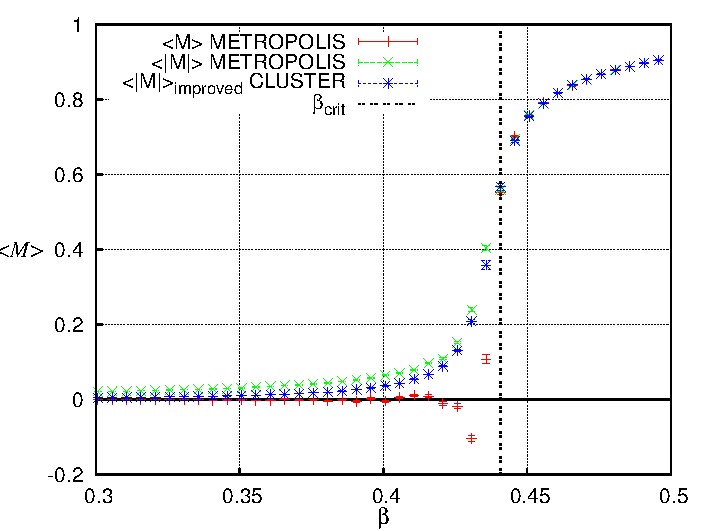
\includegraphics[scale=0.65]{Immagini/Confronto_M_andamento}
     \end{minipage}
     \begin{minipage}{0.5\textwidth}
\centering
\caption[ParteB$\_$Termal$\_$M$\_$Confronto.cpp]{\footnotesize Oscillazioni termiche }\label{fig: Confronto_M_termal}
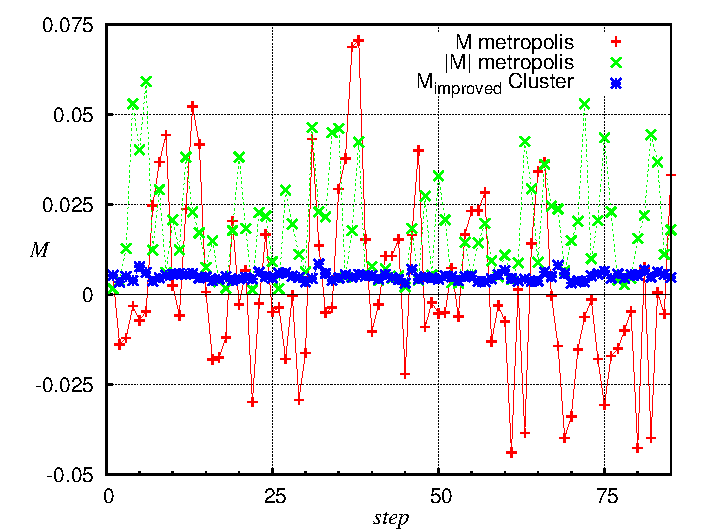
\includegraphics[scale=0.65]{Immagini/Confronto_M_termal}
     \end{minipage}
  \newline \center \footnotesize L=100, $K_{metro} = 15000$, $K_{cluster} = 1500$
\end{figure}
L'effetto è da imputare al modo differente in cui i due algoritmi simulano le fluttuazioni termiche (figura ~\ref{fig: Confronto_M_termal}).






